%%%%%%%%%%%%%%%%%%%%%%%%%%%%%%%%%%%%%%%%%
% baposter Landscape Poster
% LaTeX Template
% Version 1.0 (11/06/13)
%
% baposter Class Created by:
% Brian Amberg (baposter@brian-amberg.de)
%
% This template has been downloaded from:
% http://www.LaTeXTemplates.com
%
% License:
% CC BY-NC-SA 3.0 (http://creativecommons.org/licenses/by-nc-sa/3.0/)
%
%%%%%%%%%%%%%%%%%%%%%%%%%%%%%%%%%%%%%%%%%

%----------------------------------------------------------------------------------------
%	PACKAGES AND OTHER DOCUMENT CONFIGURATIONS
%----------------------------------------------------------------------------------------

\documentclass[a0paper,fontscale=0.32]{baposter} % Adjust the font scale/size here

\usepackage{graphicx} % Required for including images
\graphicspath{{figures/}} % Directory in which figures are stored

\usepackage{amsmath} % For typesetting math
\usepackage{amssymb} % Adds new symbols to be used in math mode
\usepackage[utf8]{inputenc}
\usepackage{booktabs} % Top and bottom rules for tables
\usepackage{enumitem} % Used to reduce itemize/enumerate spacing
\usepackage[default]{sourcesanspro} % Use the Palatino font
\usepackage[font=small,labelfont=bf]{caption} % Required for specifying captions to tables and figures

\usepackage{multicol} % Required for multiple columns
\setlength{\columnsep}{1.5em} % Slightly increase the space between columns
\setlength{\columnseprule}{0mm} % No horizontal rule between columns

\usepackage{tikz} % Required for flow chart
\usetikzlibrary{shapes,arrows} % Tikz libraries required for the flow chart in the template

\newcommand{\compresslist}{ % Define a command to reduce spacing within itemize/enumerate environments, this is used right after \begin{itemize} or \begin{enumerate}
\setlength{\itemsep}{1pt}
\setlength{\parskip}{0pt}
\setlength{\parsep}{0pt}
}

\definecolor{lightblue}{rgb}{0.145,0.6666,1} % Defines the color used for content box headers
\definecolor{grorange}{RGB}{255,93,8}

\begin{document}

\begin{poster}
{
headerborder=closed, % Adds a border around the header of content boxes
colspacing=1em, % Column spacing
bgColorOne=white, % Background color for the gradient on the left side of the poster
bgColorTwo=white, % Background color for the gradient on the right side of the poster
borderColor=black, % Border color
headerColorOne=grorange, % Background color for the header in the content boxes (left side)
headerColorTwo=grorange, % Background color for the header in the content boxes (right side)
headerFontColor=black, % Text color for the header text in the content boxes
boxColorOne=white, % Background color of the content boxes
textborder=roundedleft, % Format of the border around content boxes, can be: none, bars, coils, triangles, rectangle, rounded, roundedsmall, roundedright or faded
eyecatcher=true, % Set to false for ignoring the left logo in the title and move the title left
headerheight=0.1\textheight, % Height of the header
headershape=roundedright, % Specify the rounded corner in the content box headers, can be: rectangle, small-rounded, roundedright, roundedleft or rounded
headerfont=\Large\bf\textsc, % Large, bold and sans serif font in the headers of content boxes
%textfont={\setlength{\parindent}{1.5em}}, % Uncomment for paragraph indentation
linewidth=1pt % Width of the border lines around content boxes
}
%----------------------------------------------------------------------------------------
%	TITLE SECTION 
%----------------------------------------------------------------------------------------
%
{
\includegraphics[width=13em]{gsoc}} % First university/lab logo on the left
{\bf\textsc{The Inspector (gr-inspector)\\ \Large{Signal Analysis Toolbox for GNU Radio}}\vspace{0.5em}} % Poster title
{\textsc{Sebastian Müller, Karlsruhe Institute of Technology}} % Author names and institution
{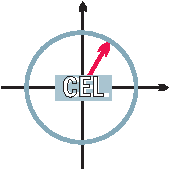
\includegraphics[width=9em]{cel}} % Second university/lab logo on the right


%----------------------------------------------------------------------------------------
%	INTRODUCTION
%----------------------------------------------------------------------------------------

\headerbox{Introduction}{name=introduction,column=0,row=0, span=1}{
gr-inspector is an out-of-tree module for GNU Radio. The target was to develop a signal analysis toolbox with the following capabilities:
\begin{itemize}\compresslist
	\item Automatic signal detection
	\item Automatic Signal Classification (AMC)
	\item OFDM parameter estimation and synchronization
	\item GUI feedback 
\end{itemize}
All these tasks should be available live during runtime.

This project was part of Google Summer of Code and ESA Summer of Code in Space programs. The toolbox was developed by Sebastian Müller
while the explicit AMC functionality was developed by Christopher Richardson.
}
	
%----------------------------------------------------------------------------------------
%	FLOWGRAPH
%----------------------------------------------------------------------------------------

\headerbox{Flowgraph}{name=flowgraph,column=1,row=0, span=2, bottomaligned=introduction}{
The toolbox was developed with the following main flowgraph in mind.

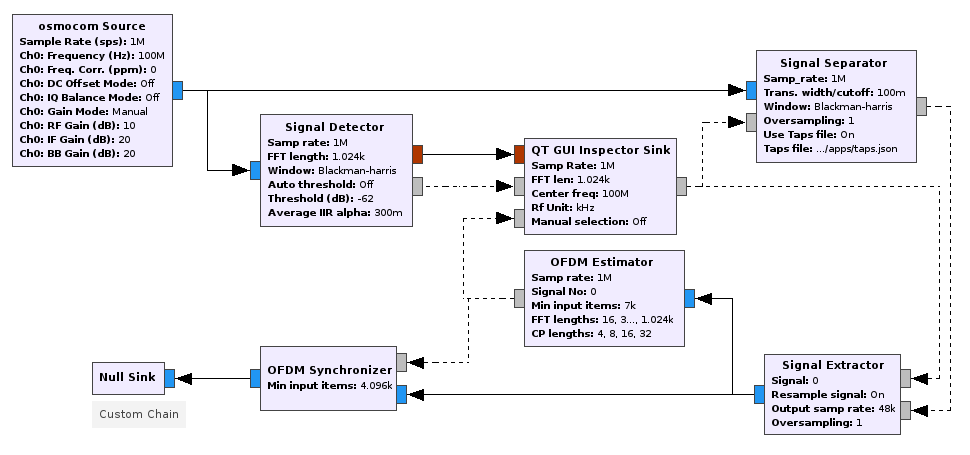
\includegraphics[width=\textwidth]{flowgraph}
\captionof{figure}{Example flowgraph}

The \textbf{Signal Extractor} block assures the ability to append custom signal processing chains for users. Each analysis block can have a feedback message to the \textbf{Inspector GUI} to print their results there.

%\vspace{0.3em} % When there are two boxes, some whitespace may need to be added if the one on the right has more content
}

%----------------------------------------------------------------------------------------
%	COMPONENTS
%----------------------------------------------------------------------------------------

\headerbox{Components}{name=components,column=0,below=introduction}{ % This block's bottom aligns with the bottom of the conclusion block
The toolbox consist of the follwing blocks:
\paragraph{Signal Detector}
Is able to perform energy detection on an input signal. The user can specify a threshold in dB or use an automatic threshold calculation by entering a sensitivity between 0 and 1.

\paragraph{Inspector GUI}
The GUI block uses QT and QWT to create a plot of the estimated PSD by the \textbf{Signal Detector} and marks the detected signal edges. By enabling manual selection, users can select own parts of the spectrum that get passed downstream. Analysis blocks can be connected to the GUI to display analysis results directly next to the specific signal.

\paragraph{Signal Separator}
Uses FIR filters for every detected/selected input signal to mix, filter and decimate this signal out of the input spectrum. All the signal samples get wrapped in a message and passed downstream. Taps can be calculated during runtime or a precalculated taps file can be selected.

\paragraph{Signal Extractor}
Takes messages from the \textbf{Signal Separator} and extracts only the samples belonging to the specified signal in the block parameters. The extracted signals get passed as a complex stream. The input samples can be resampled to satisfy a constand output sample rate.

\paragraph{AMC Block}
\textbf{TODO}

\paragraph{OFDM Estimator}
Estimates OFDM parameters subcarrier spacing, symbol time, FFT lenght and CP length.

\paragraph{OFDM Synchronizer}
After performed estimation, the signal can be frequency synchronized and stream tags can be inserted at OFDM symbol beginnings.

}
%----------------------------------------------------------------------------------------
%	MATERIALS AND METHODS
%----------------------------------------------------------------------------------------

\headerbox{Materials \& Methods}{name=method,column=0,below=components}{ % This block's bottom aligns with the bottom of the conclusion block

The following materials were required to complete the research:

\begin{itemize}\compresslist
\item Curabitur pellentesque dignissim
\item Eu facilisis est tempus quis
\item Duis porta consequat lorem
\item Eu facilisis est tempus quis
\end{itemize}

The following equations were used for statistical analysis:

\begin{equation}
\cos^3 \theta =\frac{1}{4}\cos\theta+\frac{3}{4}\cos 3\theta
\label{eq:refname}
\end{equation}\

\begin{equation}
E = mc^{2}
\label{eqn:Einstein}
\end{equation}

Phasellus imperdiet, tortor vitae congue bibendum, felis enim sagittis lorem, et volutpat ante orci sagittis mi. Morbi rutrum laoreet semper. Morbi accumsan enim nec tortor consectetur non commodo nisi sollicitudin. Proin sollicitudin. Pellentesque eget orci eros.
}

%----------------------------------------------------------------------------------------
%	MATERIALS AND METHODS
%----------------------------------------------------------------------------------------

\headerbox{Materials \& Methods}{name=method,column=1,below=components}{ % This block's bottom aligns with the bottom of the conclusion block

The following materials were required to complete the research:

\begin{itemize}\compresslist
\item Curabitur pellentesque dignissim
\item Eu facilisis est tempus quis
\item Duis porta consequat lorem
\item Eu facilisis est tempus quis
\end{itemize}

The following equations were used for statistical analysis:

\begin{equation}
\cos^3 \theta =\frac{1}{4}\cos\theta+\frac{3}{4}\cos 3\theta
\label{eq:refname}
\end{equation}\

\begin{equation}
E = mc^{2}
\label{eqn:Einstein}
\end{equation}

Phasellus imperdiet, tortor vitae congue bibendum, felis enim sagittis lorem, et volutpat ante orci sagittis mi. Morbi rutrum laoreet semper. Morbi accumsan enim nec tortor consectetur non commodo nisi sollicitudin. Proin sollicitudin. Pellentesque eget orci eros.
}

%----------------------------------------------------------------------------------------
%	GUI
%----------------------------------------------------------------------------------------

\headerbox{GUI}{name=gui, column=1, span=2, below=introduction, bottomaligned=components}{
	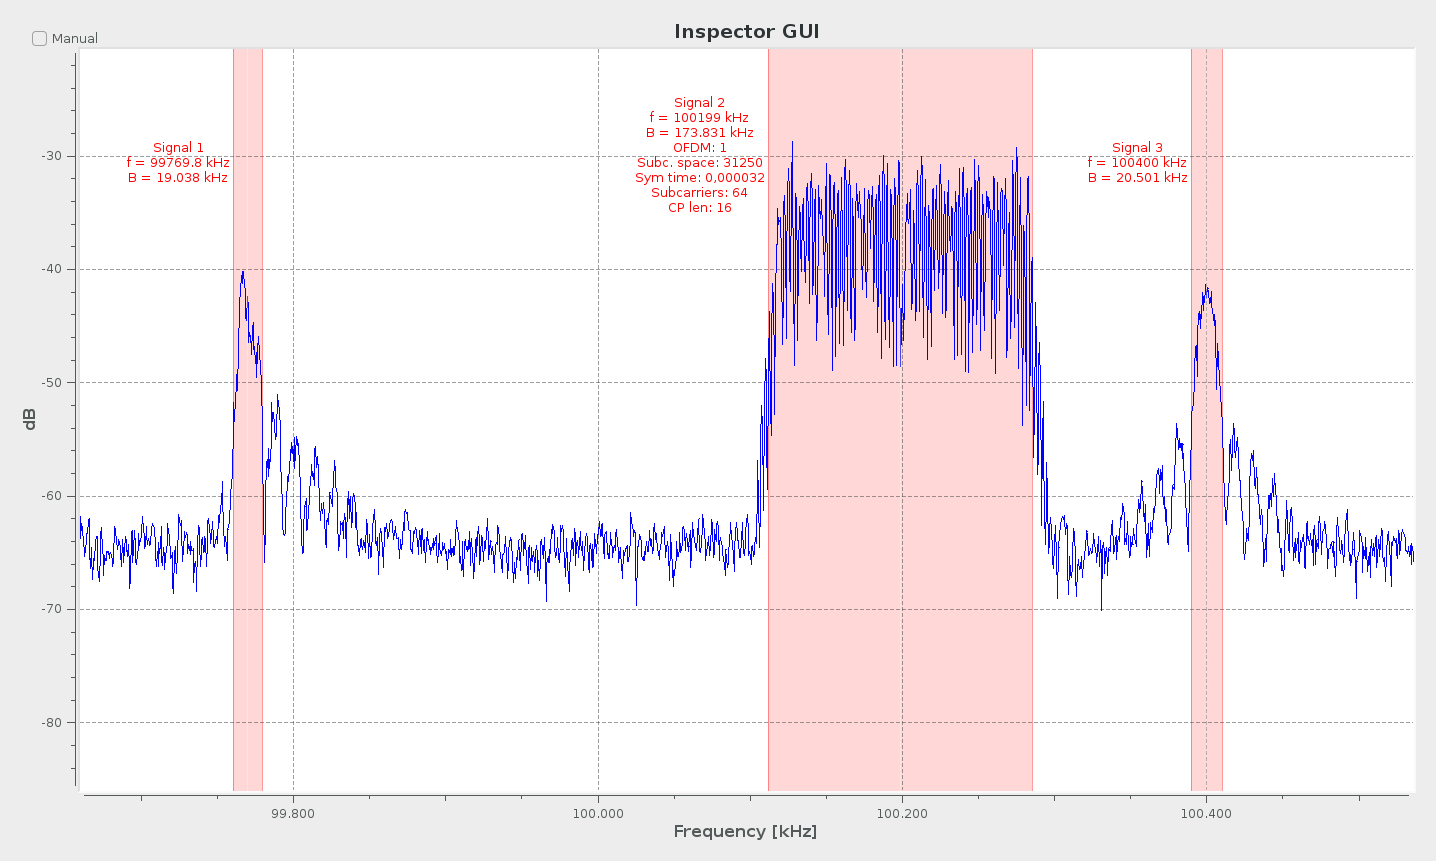
\includegraphics[width=\textwidth]{gui}
	\captionof{figure}{Inspector GUI}
}
%----------------------------------------------------------------------------------------
%	MATERIALS AND METHODS
%----------------------------------------------------------------------------------------

\headerbox{Materials \& Methods}{name=method,column=2,below=components}{ % This block's bottom aligns with the bottom of the conclusion block

The following materials were required to complete the research:

\begin{itemize}\compresslist
\item Curabitur pellentesque dignissim
\item Eu facilisis est tempus quis
\item Duis porta consequat lorem
\item Eu facilisis est tempus quis
\end{itemize}

The following equations were used for statistical analysis:

\begin{equation}
\cos^3 \theta =\frac{1}{4}\cos\theta+\frac{3}{4}\cos 3\theta
\label{eq:refname}
\end{equation}\

\begin{equation}
E = mc^{2}
\label{eqn:Einstein}
\end{equation}

Phasellus imperdiet, tortor vitae congue bibendum, felis enim sagittis lorem, et volutpat ante orci sagittis mi. Morbi rutrum laoreet semper. Morbi accumsan enim nec tortor consectetur non commodo nisi sollicitudin. Proin sollicitudin. Pellentesque eget orci eros.
}

%----------------------------------------------------------------------------------------
%	CONTACT
%----------------------------------------------------------------------------------------

\headerbox{Contact}{name=contact,column=2,above=bottom}{ % This block is as tall as the references block
Maintainers of this module:
\begin{multicols}{2}
Sebastian Müller\\
KIT Karlsruhe\\
gsenpo@gmail.com

Christopher Richardson\\
Lancaster University\\
c.richardson@lancaster.ac.uk
\end{multicols}

}

%----------------------------------------------------------------------------------------
%	REFERENCES
%----------------------------------------------------------------------------------------

\headerbox{References}{name=references,column=0,span=2, above=bottom, aligned=contact}{

\renewcommand{\section}[2]{\vskip 0.05em} % Get rid of the default "References" section title
\nocite{*} % Insert publications even if they are not cited in the poster
\small{ % Reduce the font size in this block
\bibliographystyle{unsrt}
\bibliography{sample} % Use sample.bib as the bibliography file
}}




%----------------------------------------------------------------------------------------

\end{poster}

\end{document}
